\documentclass{beamer}
\usepackage{ucltemplate}

%% Choose the color you like
\usecolortheme{blue}
\setbeamertemplate{navigation symbols}{}

%\AtBeginSection[] {
%  \begin{frame}
%    \frametitle{Outline}
%    \tableofcontents[currentsection]
%  \end{frame}
%}

%\usepackage[colorlinks=true]{hyperref}

\title{Variant calling and annotation}
\author[]{Vincent Plagnol}
\institute{
Inivata- Head of Computational Biology\\
UCL- Reader in Statistical Genetics\\
}
\date{}


\begin{document}

\maketitle


\begin{frame}
  \frametitle{Outline}
  \tableofcontents
\end{frame}



%%%%%%%%%%%%%%%%%%%%%%%


\section{Variant calling algorithms and strategies}


\begin{frame}
  \frametitle{There are several calling algorithms available to you}
  \begin{itemize}
  \item \texttt{samtools} has a perfectly valid variant calling algorithm.
  \item \texttt{GATK} is usually considered the gold standard but there are several ways to use it, which we will discuss today.
  \item Other options include the recently release \texttt{platypus}.
  \end{itemize}
\end{frame}


\begin{frame}
  \frametitle{Why calling each sample individually is not always a great idea}
  \begin{itemize}
  \item When one works genome-wide, there are always artifacts and technical issues to deal with.
  \item Sometimes you see the same ``rare variant'' coming up across multiple smaples.
    \begin{itemize}
    \item This is obviously extremely unlikely to happen.
    \end{itemize}
  \item Looking at multiple samples can point to these errors and help you better understand the data.
  \end{itemize}
\end{frame}

\begin{frame}
  \frametitle{One can also gain power}
  \begin{center}
    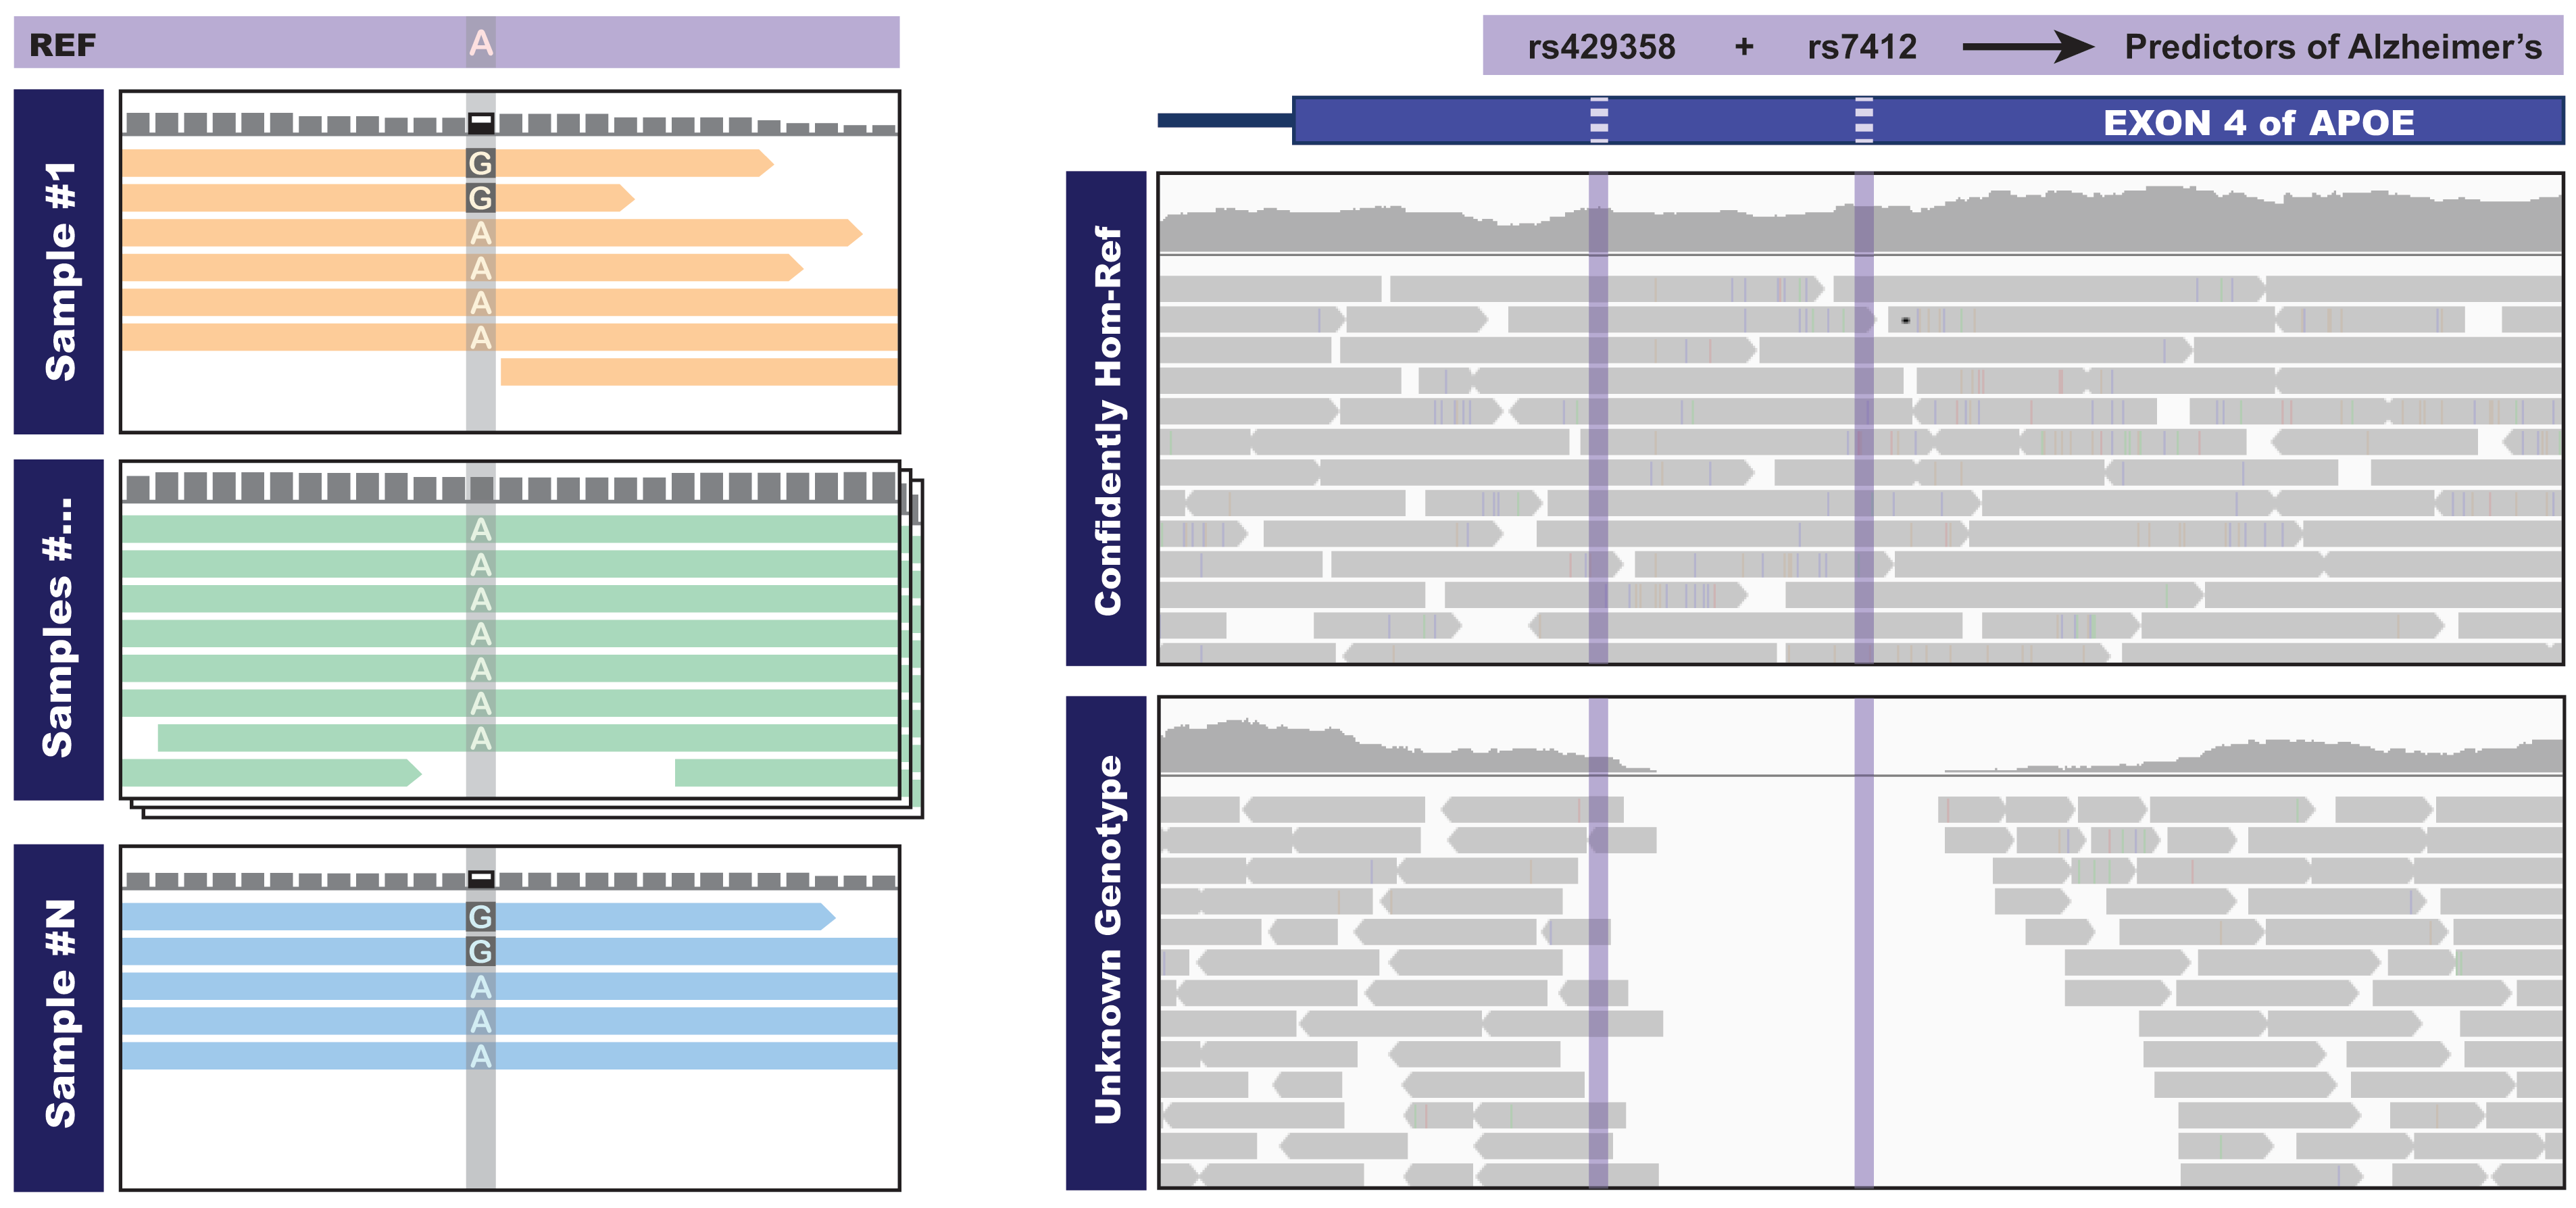
\includegraphics[width=11cm]{fig/joint_calling.png}
  \end{center}
\end{frame}


\begin{frame}
  \frametitle{A bit of history: the reduceReads format}
  \begin{center}
    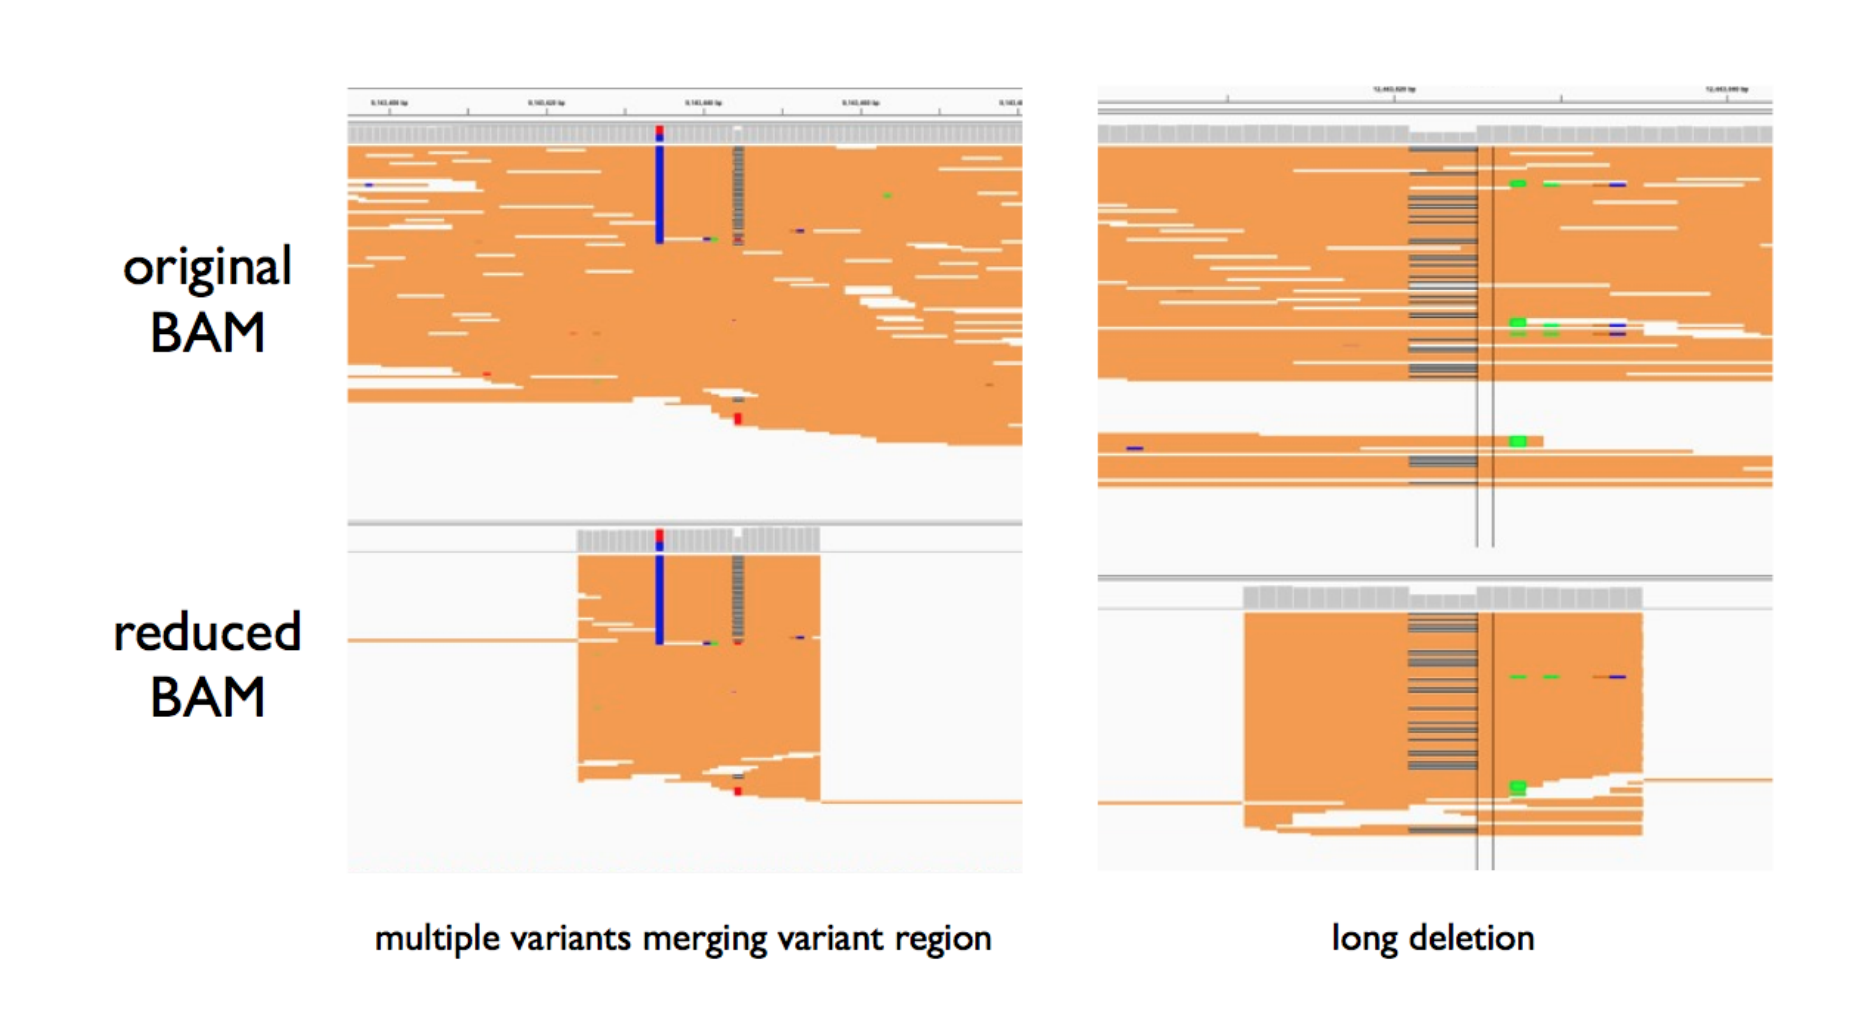
\includegraphics[width=11cm]{fig/reducedReads.png}
  \end{center}
\end{frame}


\begin{frame}
  \frametitle{Why is this a hard problem?}
  \begin{itemize}
  \item We all agree that we do not want to process 20 Tb of exomes each time we add one extra sample.
  \item But then, what is the intermediate step?
  \item We must know not only the variant called, but also the regions where there are NO variant call.
  \item And when there is a hint of a call, we must also remember that.
    \begin{itemize}
    \item This is really a compression problem.
    \end{itemize}
  \end{itemize}
\end{frame}

\begin{frame}
  \frametitle{The drawback of multi-sample calling}
  \begin{itemize}
  \item The computational challenges can be daunting: can you process together 50,000 samples?
  \item There is also a (N+1) problem: this one extra sample you forgot to process may cost you 1,000 hours of computing.
  \item To mitigate these issues, the GATK team has put together a hybrid concept, the gVCF workflow that we will look at today.
  \end{itemize}
\end{frame}

\begin{frame}
  \frametitle{Joint vs single sample calling}
  \begin{center}
    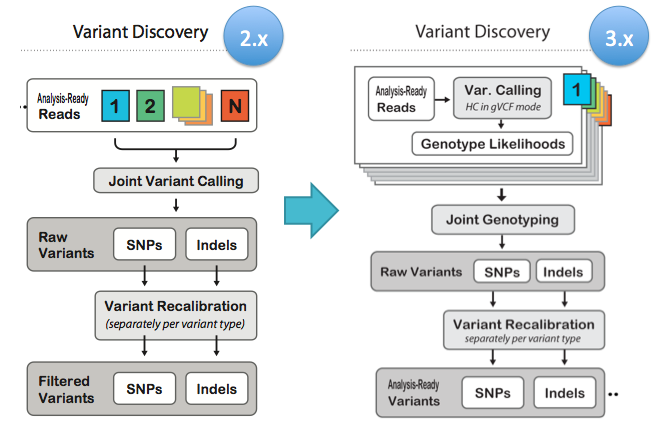
\includegraphics[width=8cm]{fig/joint_vs_single_calling.png}
  \end{center}
\end{frame}

\begin{frame}
  \frametitle{A consequence: massive centralized variant calling efforts}
  \begin{itemize}
  \item Given the strong gain in power it really makes sense to have centralized teams handling the calling.
  \item The most obvious example is the Broad theme (Boston) and the release of the ExAC calls.
    \begin{itemize}
    \item This \href{http://exac.broadinstitute.org/}{website} is a ``must visit'' for anyone working on human genetics.
    \item You will find about 80,000 exomes jointly called.
    \item It gives an extraordinary perspective on coding regions variability.
    \end{itemize}
  \end{itemize}
\end{frame}


\begin{frame}
  \frametitle{New kids in town}
  \begin{itemize}
  \item \href{http://www.nature.com/nmeth/journal/vaop/ncurrent/full/nmeth.3505.html}{SpeedSeq} is supposed to work well.
  \item All these tools try to find a balance between accuracy and speed.
  \item Projets like Genomics England really struggle with computational burden and are interested in solutions that are faster than GATK.
  \item \texttt{Platypus} is another new tool from the Oxford group.
  \end{itemize}
\end{frame}


\begin{frame}
  \frametitle{My bit of advice}
  \begin{itemize}
    \item Think very carefully about your headers, and how you name samples.
    \item If you get this wrong, it is very hard to fix.
    \item Also think about your reference genome. Once a choice is made, there is hardly a way back.
  \end{itemize}
\end{frame}


%%%%%%%%%%%%%%%%%%%%%%%
\section{Variant calling format}

\begin{frame}
  \frametitle{The variant calling format (VCF)}
  \begin{itemize}
  \item The VCF format is now supported by a team from the ``Global Alliance for Genomics and Health''.
  \item A link to file formats can be found \href{http://ga4gh.org/\#/fileformats-team}{at this location}.
  \item I am not yet familiar with this website but I am hoping that much will happen there, we need this to be successful.
  \end{itemize}
\end{frame}


\begin{frame}
  \frametitle{The variant calling format}
  \begin{itemize}
  \item This is an incredibly loosely defined format.
  \item A colleague argued that at the core, it's really just a bunch of tab delimited columns.
  \item And in particular \texttt{samtools} and \texttt{GATK} will output slightly different things.
  \item Nevertheless, the VCF format is ubiquitous and it is important to understand what it stores.
  \end{itemize}
\end{frame}



\begin{frame}
  \frametitle{An exercise to go through together}
  \begin{itemize}
  \item Compare the flavours of VCF format between \texttt{samtools} and \texttt{GATK}.
  \item Note the genotype likelihood, stored in Phred scaled format.
  \item See what GATK shows that \texttt{samtools} does not show.
  \end{itemize}
\end{frame}
    


%%%%%%%%%%%%%
\section{Annotating your variants}

\begin{frame}
  \begin{itemize}
  \frametitle{This is not easy!}
  \item Different tools can give you very different interpretations.
    \begin{itemize}
    \item The primary issue is differences in the underlying database.
    \item A second issue is the handling of the multiple transcripts for each gene.
    \item And the third issue is the actual data analysis, with potential minor bugs.
    \end{itemize}
  \item I have used a lot \href{http://annovar.openbioinformatics.org/en/latest/}{ANNOVAR} in the past...
  \item ... but really the variant effect predictor (VEP) is a better tool.
  \end{itemize}
\end{frame}


\begin{frame}
  \frametitle{More on annotations}
  \begin{itemize}
  \item Think carefully about the annotation database that you use.
  \item Mare careful choices about the way you handle multiple transcripts.
  \end{itemize}
\end{frame}

\end{document}
